% move all configuration stuff into one file so we can focus on the content
\documentclass[aspectratio=169,hyperref={pdfpagelabels=false,colorlinks=true,linkcolor=white,urlcolor=lightblue},xcolor={table},t]{beamer}

%%%%%%%%%%%%%%%%%%%%%%%%%%%%%%%%%%%%%%%%%%%%%%%%%%%%%%%%%%%%%%%%%%%%%%%%%%%%%%%%%%
%%%%%%%%%%%%%%%%%%%%%%%%%%%%%%%%%%%%%%%%%%%%%%%%%%%%%%%%%%%%%%%%%%%%%%%%%%%%%%%%%%
% packages
\usepackage{pict2e}
\usepackage{epic}
\usepackage{amsmath,amsfonts,amssymb}
\usepackage{units}
\usepackage{fancybox}
\usepackage[absolute,overlay]{textpos} 
%\usepackage[table]{xcolor}
\usepackage{animate}
\usepackage{gensymb}
%\usepackage{graphicx}
%\usepackage{longtable}
\usepackage{multirow}
\usepackage{silence}
\usepackage{tikz}
\usepackage[backend=bibtex,style=ieee]{biblatex}
\AtEveryCitekey{\iffootnote{\tiny}{}}
%\addbibresource{include/references}



% fontsize
\let\Tiny=\tiny

%%%%%%%%%%%%%%%%%%%%%%%%%%%%%%%%%%%%%%%%%%%%%%%%%%%%%%%%%%%%%%%%%%%%%%%%%%%%%%%%%%
%%%%%%%%%%%%%%%%%%%%%%%%%%%%%%%%%%%%%%%%%%%%%%%%%%%%%%%%%%%%%%%%%%%%%%%%%%%%%%%%%%
% warnings
\pdfsuppresswarningpagegroup=1
\WarningFilter{biblatex}{Patching footnotes failed}
\WarningFilter{latexfont}{Font shape}
\WarningFilter{latexfont}{Some font shapes}
\WarningFilter{gensymb}{Not defining}


%%%%%%%%%%%%%%%%%%%%%%%%%%%%%%%%%%%%%%%%%%%%%%%%%%%%%%%%%%%%%%%%%%%%%%%%%%%%%%%%%%
%%%%%%%%%%%%%%%%%%%%%%%%%%%%%%%%%%%%%%%%%%%%%%%%%%%%%%%%%%%%%%%%%%%%%%%%%%%%%%%%%%
% colors
\definecolor{gtgold}{rgb}{.914, .664, 0} %0e7eed {rgb}{0.88,0.66,1,0.06} [234, 170, 0]/256 %96caff
\definecolor{darkgray}{rgb}{.15, .15, .15}
\definecolor{lightblue}{HTML}{0e7eed}
\definecolor{highlight}{rgb}{0, 0, 1} %_less!40

%%%%%%%%%%%%%%%%%%%%%%%%%%%%%%%%%%%%%%%%%%%%%%%%%%%%%%%%%%%%%%%%%%%%%%%%%%%%%%%%%%
%%%%%%%%%%%%%%%%%%%%%%%%%%%%%%%%%%%%%%%%%%%%%%%%%%%%%%%%%%%%%%%%%%%%%%%%%%%%%%%%%%
% relative paths
\graphicspath{{../graph/}}


%%%%%%%%%%%%%%%%%%%%%%%%%%%%%%%%%%%%%%%%%%%%%%%%%%%%%%%%%%%%%%%%%%%%%%%%%%%%%%%%%%
%%%%%%%%%%%%%%%%%%%%%%%%%%%%%%%%%%%%%%%%%%%%%%%%%%%%%%%%%%%%%%%%%%%%%%%%%%%%%%%%%%
% units
\setlength{\unitlength}{1mm}

%%%%%%%%%%%%%%%%%%%%%%%%%%%%%%%%%%%%%%%%%%%%%%%%%%%%%%%%%%%%%%%%%%%%%%%%%%%%%%%%%%
%%%%%%%%%%%%%%%%%%%%%%%%%%%%%%%%%%%%%%%%%%%%%%%%%%%%%%%%%%%%%%%%%%%%%%%%%%%%%%%%%%
% math
\DeclareMathOperator*{\argmax}{argmax}
\DeclareMathOperator*{\argmin}{argmin}
\DeclareMathOperator*{\atan}{atan}
\DeclareMathOperator*{\arcsinh}{arcsinh}
\DeclareMathOperator*{\sign}{sign}
\DeclareMathOperator*{\tcdf}{tcdf}
\DeclareMathOperator*{\si}{sinc}
\DeclareMathOperator*{\princarg}{princarg}
\DeclareMathOperator*{\arccosh}{arccosh}
\DeclareMathOperator*{\hwr}{HWR}
\DeclareMathOperator*{\flip}{flip}
\DeclareMathOperator*{\sinc}{sinc}
\DeclareMathOperator*{\floor}{floor}
\newcommand{\e}{{e}}
\newcommand{\jom}{\mathrm{j}\omega}
\newcommand{\jOm}{\mathrm{j}\Omega}
\newcommand   {\mat}[1]    		{\boldsymbol{\uppercase{#1}}}		%bold
\renewcommand {\vec}[1]    		{\boldsymbol{\lowercase{#1}}}		%bold

%%%%%%%%%%%%%%%%%%%%%%%%%%%%%%%%%%%%%%%%%%%%%%%%%%%%%%%%%%%%%%%%%%%%%%%%%%%%%%%%%%
%%%%%%%%%%%%%%%%%%%%%%%%%%%%%%%%%%%%%%%%%%%%%%%%%%%%%%%%%%%%%%%%%%%%%%%%%%%%%%%%%%
% media9
\newcommand{\includeaudio}[1]{
\href{run:audio/#1.mp3}{
\includegraphics[width=5mm, height=5mm]{graph/SpeakerIcon}}}

\newcommand{\includeanimation}[4]{{\begin{center}
                        \animategraphics[autoplay,loop,scale=.7]{#4}{animation/#1-}{#2}{#3}        
                        \end{center}
                        \addreference{matlab source: \href{https://github.com/alexanderlerch/ACA-Plots/blob/master/matlab/animate#1.m}{matlab/animate#1.m}}}
                        \inserticon{video}}
                        
%%%%%%%%%%%%%%%%%%%%%%%%%%%%%%%%%%%%%%%%%%%%%%%%%%%%%%%%%%%%%%%%%%%%%%%%%%%%%%%%%%
%%%%%%%%%%%%%%%%%%%%%%%%%%%%%%%%%%%%%%%%%%%%%%%%%%%%%%%%%%%%%%%%%%%%%%%%%%%%%%%%%%
% other commands
\newcommand{\question}[1]{%\vspace{-4mm}
                          \setbeamercovered{invisible}
                          \begin{columns}[T]
                            \column{.9\textwidth}
                                \textbf{#1}
                            \column{.1\textwidth}
                                \vspace{-8mm}
                                \begin{flushright}
                                     
\includegraphics[width=.9\columnwidth]{graph/question_mark}
                                \end{flushright}
                                \vspace{6mm}
                          \end{columns}\pause\vspace{-12mm}}

\newcommand{\toremember}[1]{
                        \inserticon{lightbulb}
                        }

\newcommand{\matlabexercise}[1]{%\vspace{-4mm}
                          \setbeamercovered{invisible}
                          \begin{columns}[T]
                            \column{.8\textwidth}
                                \textbf{matlab exercise}: #1
                            \column{.2\textwidth}
                                \begin{flushright}
                                     \includegraphics[scale=.5]{graph/logo_matlab}
                                \end{flushright}
                                %\vspace{6mm}
                          \end{columns}}

\newcommand{\addreference}[1]{  
                  
                    \begin{textblock*}{\baselineskip }(.98\paperwidth,.5\textheight) %(1.15\textwidth,.4\textheight)
                         \begin{minipage}[b][.5\paperheight][b]{1cm}%
                            \vfill%
                             \rotatebox{90}{\tiny {#1}}
                        \end{minipage}
                   \end{textblock*}
                    }
                    
\newcommand{\figwithmatlab}[1]{
                    \begin{figure}
                        \centering
                        \includegraphics[scale=.7]{#1}
                        %\label{fig:#1}
                    \end{figure}
                    
                    \addreference{matlab source: \href{https://github.com/alexanderlerch/MUSI-6202/blob/main/matlab/plot#1.m}{plot#1.m}}}
\newcommand{\figwithref}[2]{
                    \begin{figure}
                        \centering
                        \includegraphics[scale=.7]{#1}
                        \label{fig:#1}
                    \end{figure}
                    
                    \addreference{#2}}  
                                    
\newcommand{\inserticon}[1]{
                    \begin{textblock*}{100mm}(14.5cm,7.5cm)
                        \includegraphics[height=.8cm,keepaspectratio]{graph/#1}
                    \end{textblock*}}            

%%%%%%%%%%%%%%%%%%%%%%%%%%%%%%%%%%%%%%%%%%%%%%%%%%%%%%%%%%%%%%%%%%%%%%%%%%%%%%%%%%
%%%%%%%%%%%%%%%%%%%%%%%%%%%%%%%%%%%%%%%%%%%%%%%%%%%%%%%%%%%%%%%%%%%%%%%%%%%%%%%%%%
% counters
\newcounter{i}
\newcounter{j}
\newcounter{iXOffset}
\newcounter{iYOffset}
\newcounter{iXBlockSize}
\newcounter{iYBlockSize}
\newcounter{iYBlockSizeDiv2}
\newcounter{iXBlockSizeDiv2}
\newcounter{iDistance}

\newcommand{\IEEELink}{https://ieeexplore.ieee.org/servlet/opac?bknumber=9965970}



\subtitle{Part 5: Signal Similarity --- Correlation}

%%%%%%%%%%%%%%%%%%%%%%%%%%%%%%%%%%%%%%%%%%%%%%%%%%%%%%%%%%%%%%%%%%%%%%%%%%%%
\begin{document}
    % generate title page
	\title[]{Digital Signal Processing for Music}   
\author[alexander lerch]{alexander lerch} 
%\institute{~}
%\date[Alexander Lerch]{}
\titlegraphic{\vspace{-16mm}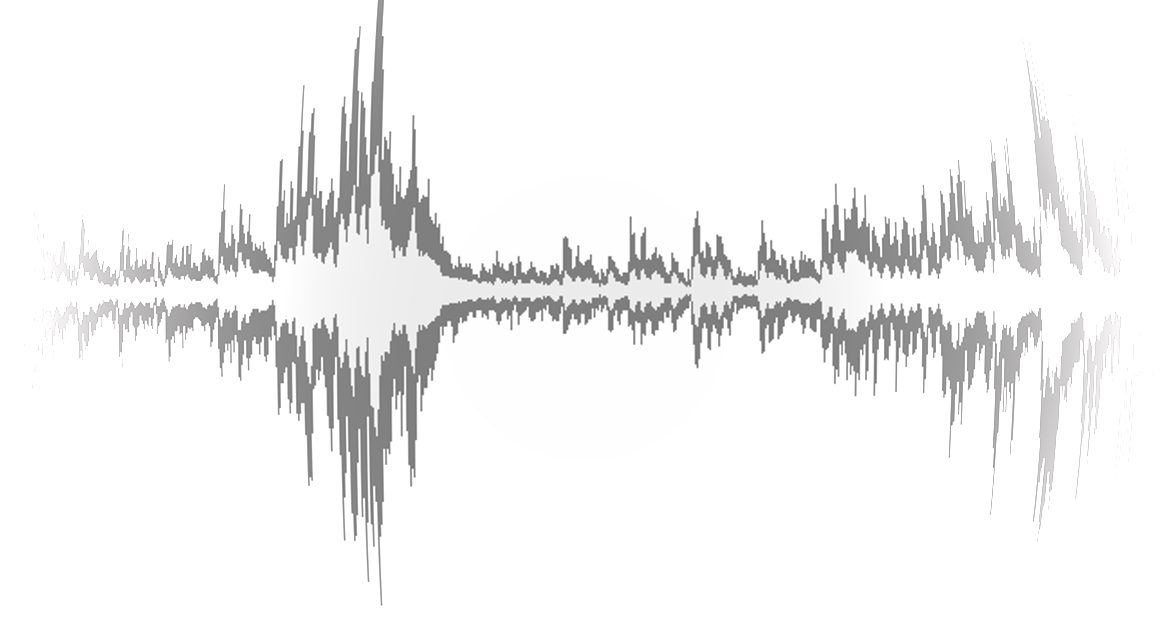
\includegraphics[width=\textwidth,height=3cm]{title}}


\begin{frame}
    \titlepage
    %\vspace{-5mm}
    \begin{flushright}
        \href{http://www.gtcmt.gatech.edu}{
\includegraphics[height=.8cm,keepaspectratio]{../shared/Logo_GTCMT_black}}
    \end{flushright}
\end{frame}


\section{introduction}
\begin{frame}{signal similarity}{introduction}
    \begin{itemize}
        \item   correlation function
            \begin{itemize}
                \item   indicates (linear) dependencies between two signals
                \item   shifts the signals to find the dependency for each shift in time
            \end{itemize}
    \end{itemize}
\end{frame}

\section{CCF}

\begin{frame}{signal similarity}{correlation function}
	compute similarity between two \textbf{stationary} signals $x$,$y$
    \begin{equation*}
        r_\mathrm{xy}(\tau)=\mathcal{E}\lbrace x(t)y(t+\tau)\rbrace  
    \end{equation*}  
	\pause
    
	\begin{itemize}
		\item	\textbf{continuous}:
            \begin{equation*}
                r_\mathrm{xy}(\tau) = \int\limits_{-\infty}^{\infty}{x(t)\cdot y(t+\tau)dt}
            \end{equation*}
		\item	\textbf{discrete}:
            \begin{equation*}
                r_\mathrm{xy}(\eta) = \sum\limits_{i=-\infty}^{\infty}{x(i)\cdot y(i+\eta)}
            \end{equation*}
	\end{itemize}
\end{frame}

\begin{frame}{signal similarity}{correlation function: animation}
    \vspace{-5mm}
    \begin{footnotesize}
    \begin{equation*}
        r_\mathrm{xy}(\tau) = \int\limits_{-\infty}^{\infty}{x(t)\cdot y(t+\tau)}dt
    \end{equation*}
    \end{footnotesize}
    \includevideo{XCorrAnimation}
\end{frame}

\begin{frame}{signal similarity}{correlation function: use cases}
    \begin{itemize}
        \item   find (linear!) similarity between two signals (e.g., clean and noisy)
        \item   find time shift between to similar signals
        \pause
        \bigskip
        \item   example: \textbf{radar}
            \begin{itemize}
                \item   correlate sent signal with received signal
                \item   pick maximum location and convert to distance of object
            \end{itemize}
    \end{itemize}
\end{frame}

\section[correlation coefficient]{normalized correlation and correlation coefficient}
\begin{frame}{signal similarity}{correlation coefficient}
    \begin{equation*}\nonumber
        r_\mathrm{xy}(\tau) = \frac{\mathcal{E}\lbrace(X-\mu_X)(Y-\mu_Y)\rbrace}{\sigma_X\sigma_Y}
    \end{equation*}
    
    special case: \textbf{Pearson Correlation Coefficient} $r_\mathrm{xy}(0)$ after normalization
    \bigskip
    \bigskip
    \question{What are possible reasons for normalization}
        \begin{itemize}
            \item   ensuring that function will always be between -1 and 1
            \item   shifting and scaling one signal will not change the coefficient
        \end{itemize}
\end{frame}

\section{possible issues}
\begin{frame}{signal similarity}{correlation function: problems as summary statistic}
Anscombe's quartet:
    \begin{itemize}
        \item   identical mean: 7.5
        \item   identical variance: 4.2
        \item   identical \textbf{Pearson correlation coefficient}: 0.816
    \end{itemize}
    \begin{figure}
        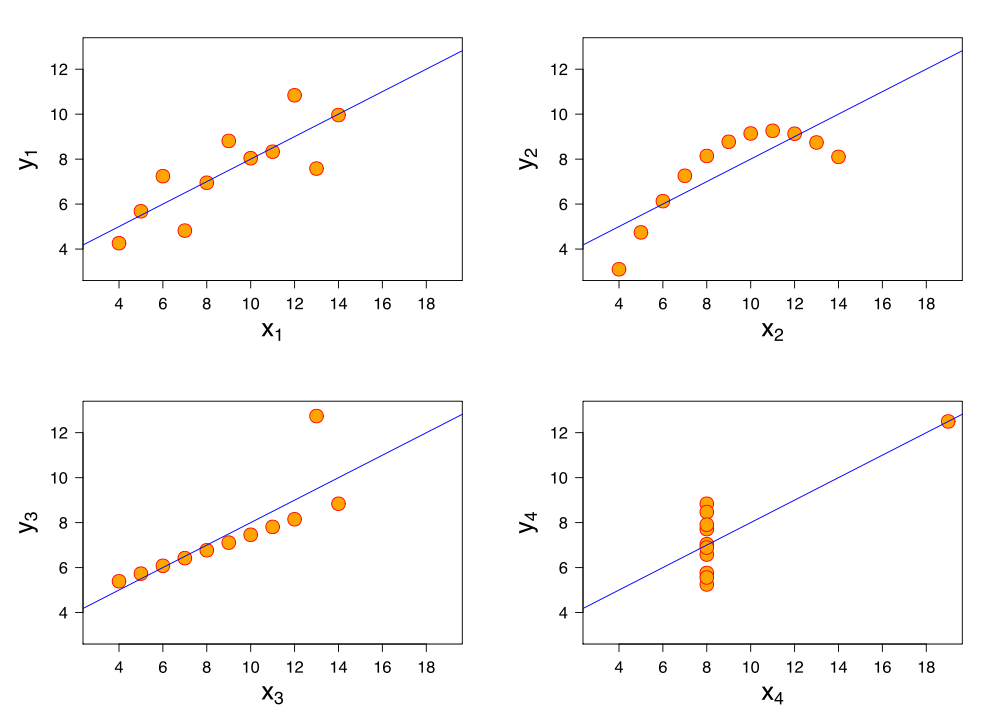
\includegraphics[scale=.2]{graph/Anscombes_quartet}
    \end{figure}
\end{frame}

\section{examples}
\begin{frame}\frametitle{correlation function}\framesubtitle{examples 1/3}
		\question{Describe the (cross) correlation function between the following signals}
			
		\begin{itemize}
			\item	rectangular window vs.
			\item	windowed sine vs.
			\item	noise
		\end{itemize}
\end{frame}

\begin{frame}\frametitle{correlation function}\framesubtitle{examples 2/3}
    \vspace{-5mm}
    \begin{figure}
        \centering
            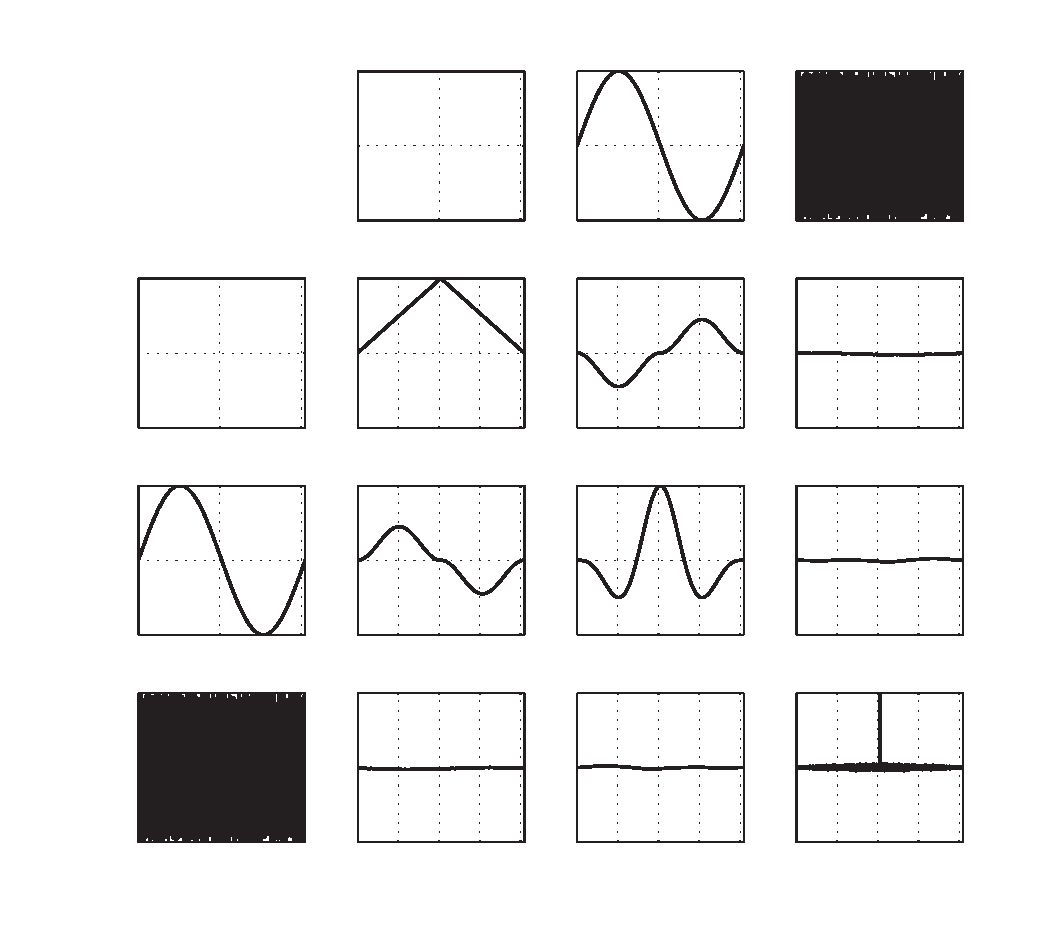
\includegraphics[scale=.5]{graph/xcorr}
        \label{fig:xcorr}
    \end{figure}
\end{frame}

\begin{frame}\frametitle{correlation function}\framesubtitle{animation}
            \vspace{-5mm}
            \begin{footnotesize}
                    \begin{equation*}
                        %r_\mathrm{xy}(\tau) &=& \int\limits_{-\infty}^{\infty}{x(t)\cdot y(t+\tau)dt}\\
                        r_\mathrm{xy}(\eta) = \sum\limits_{i=-\infty}^{\infty}{x(i)\cdot y(i+\eta)}
                    \end{equation*}
            \end{footnotesize}
            \begin{center}
                \animategraphics[loop]{10}{animateCorrelation/Correlation-}{000}{250}        
            \end{center}
            \addreference{matlab source: \href{https://github.com/alexanderlerch/ACA-Slides/blob/master/matlab/animateCorrelation.m}{matlab/animateCorrelation.m}}
            \inserticon{video}
\end{frame}	
        \begin{frame}{correlation function}{blocked correlation: animation}
            \begin{center}
                \animategraphics[loop]{24}{animateBlockedCorrelation/BlockedCorrelation-}{001}{1023}        
            \end{center}
            \addreference{matlab source: \href{https://github.com/alexanderlerch/ACA-Slides/blob/master/matlab/animateBlockedCorrelation.m}{matlab/animateBlockedCorrelation.m}}
            \inserticon{video}
        \end{frame}	 

\section{ACF}
\begin{frame}{correlation function}{auto correlation function}
		\begin{equation*}
			r_\mathrm{xx}(\tau)=\mathcal{E}\lbrace x(t)x(t+\tau)\rbrace  
		\end{equation*}

		\pause
		\begin{block}{autocorrelation function properties}
			\begin{itemize}
				\item	\textbf{power}: $r_{xx}(0) = 	\mathcal{E}\lbrace X^2\rbrace $ 

				\smallskip
				\item<2->	\textbf{symmetry} $r_{xx}(\tau)=r_{xx}(-\tau)$\\
					(substitute $t=t'+\tau$)

				\smallskip
                \item<3->	\textbf{global max}: $r_{xx}(\tau)\leq r_{xx}(0)$ 
					%(Binomial theorem $E\left\lbrace \big(x(t)x(t-\tau)\big)^2\right\rbrace $ )

				\smallskip
				\item<4->	\textbf{periodicity}:\\
					The {ACF} of a periodic signal is periodic (period length of input signal)

			\end{itemize}	
		\end{block}
\end{frame}	

%\begin{frame}{correlation and power spectral density}{PSD}
	%\begin{itemize}
		%\item	\textbf{problem}: how to calculate the spectrum of a random process?
				%\begin{itemize}
					%\item	no analytic function to integrate
				%\end{itemize}
				%
		%\pause
		%\item	\textbf{solution}: Wiener-Khinchin theorem
		%\pause
		%\begin{equation*}
			%S_{xx}(\omega) = \mathfrak{F}\lbrace \varphi_{xx}(\tau)\rbrace 
		%\end{equation*}
	%\end{itemize}
%\end{frame}
%
%\begin{frame}{correlation and power spectral density}{PSD: properties}
%
		%\begin{block}{PSD properties}
			%\begin{itemize}
				%\item	\textbf{real} (symmetry in time domain!) 
%
				%\pause
				%\item	\textbf{power preservation}
					%\begin{equation*}
						%\mathcal{E}\lbrace x^2\rbrace  = \varphi_{xx}(\tau = 0) = \frac{1}{2\pi}\int\limits_{-\infty}^{\infty}{S_{xx}(\omega)\enspace d\omega} 
					%\end{equation*}
			%\end{itemize}	
		%\end{block}
%\end{frame}	
%
%\begin{frame}{correlation and power spectral density}{PSD: discrete signals}
	%\begin{itemize}
		%\item	\textbf{correlation}
				%\begin{equation*}
					%\varphi_{xx}(l) = \mathcal{E}\lbrace x(n)\cdot x(n-l)\rbrace 
				%\end{equation*}
		%\pause
		%\item	\textbf{PSD}
				%\begin{equation*}
					%\varphi_{xx}(l) = \mathfrak{F^{-1}}\lbrace S_{xx}(\Omega)\rbrace =\frac{1}{2\pi}\int\limits_{-\pi}^{+\pi}S_{xx}(\Omega)e^{j\Omega l}\enspace d\Omega
				%\end{equation*}  
		%\pause
		%\item	\textbf{power}
				%\begin{equation*}
					%\varphi_{xx}(0)=\frac{1}{2\pi}\int\limits_{-\pi}^{+\pi}S_{xx}(\Omega)\enspace d\Omega
				%\end{equation*}
	%\end{itemize}
%\end{frame}	


\section{summary}
\begin{frame}{correlation function}{summary}
    \begin{itemize}
        \item   correlation function is useful tool to
            \begin{itemize}
                \item   \textbf{determine the similarity} between two signals (CCF)
                \item   \textbf{identify a shift/latency} between two similar signals (CCF)
                \item   \textbf{identify periodicity} vs. noisiness in a signal (ACF)
            \end{itemize}
        \smallskip
        \item<2->   continues to be standard approach for all applications related to the above tasks
        \smallskip
        \item<3->   note: CCF or ACF do not display time information (lost in integration)
    \end{itemize}
\end{frame}		

    
\end{document}

